\paragraph{Target applicative setup.}
To acquire plant images in a real world application scenario, we use a home made solution as a 3D
scanner. It consists in a X-Carve~\cite{xcarve} CNC Cartesian arm, combined with a
custom-made pan-tilt camera mount. This setup therefore has five degrees of freedom.
A Sony RX0 \alien{RGB }{}camera \alien{with $1920 \times 1060$ resolution}{} is mounted on the camera mount and is controlled using a Wifi interface. This allows for views from any point in space in a box containing
the imaged plant. The set-up in presented in \cite{wintz_automated_nodate}.

\paragraph{Virtual plants.}

The \tim{generative plant models}{virtual plants} were designed with
OpenAlea~\cite{pradal2009plantgl}. OpenAlea is an open source software
suite developped by INRIA to provide tools for plant architecture
modelling. \tim{The model plant \emph{Arabidopsis Thaliana} was chosen to
illustrate the methods in the paper, because it is a well-studied
plant and is a subject of active interest for many biologists.}{}

\tim{A generative model of \emph{A. Thaliana} was specifically
written in the L-py programming language. L-py is a python extension,
part of OpenAlea, which implements L-systems.}{3D meshes of \emph{A.
Thaliana} were designed with the L-Py library from OpenAlea, which
is a python implementation of L-system.} L-systems were developped
in 1968 by Aristid Lindenmayer~\cite{prusinkiewicz2012algorithmic}
to model plant growth.  It is a generative grammar that allows to
grow a virtual plant using symbols, shapes and constraints derived
\tim{from}{for} plant growth observation.

Formally it is called a rewriting system, or formal grammar. It
comprises:

\begin{itemize}
    \item A vocabulary V containing the \emph{modules} of the
    system. For plant generation it will represent an architectural
    element of the plant (apex, internode, leaf) and associated
    parameters (age, length, etc) \item An initial \emph{axiom}
    or state $s_0$ corresponding to the virtual plant at $t_0$. It
    is a string of elements from the vocabulary.  \item A set
    of \emph{production} rules to iterate in order to model
    the growth. They will be applied in parallel to each variable
    element from the string of the previous state. They are composed
    of a \emph{predecessor}, to identify the elements that will be
    replaced by a \emph{successor}.
\end{itemize}

\tim{Randomness can be added to the models by assigining different
probabilities to the set for rules. This allow to produce different
looking individual plants from a single set of rules. \alien{}{Our L-py model
for \emph{A. Thaliana} can be found online \cite{Lpy_godin}.}}{}

The strings can then be represented graphically in 3D using OpenAlea's
PlantGL (Figure\ref{fig:lpy}). Figure~\ref{fig:lpy} illustrates a virtual specimen
of A. Thaliana obtained using the lpy generative model at different timesteps.

The A. Thaliana models comprised 5 different types of organs: fruit, stem, pedicel, leaf and flower.

\begin{figure}[h!]
    \centering 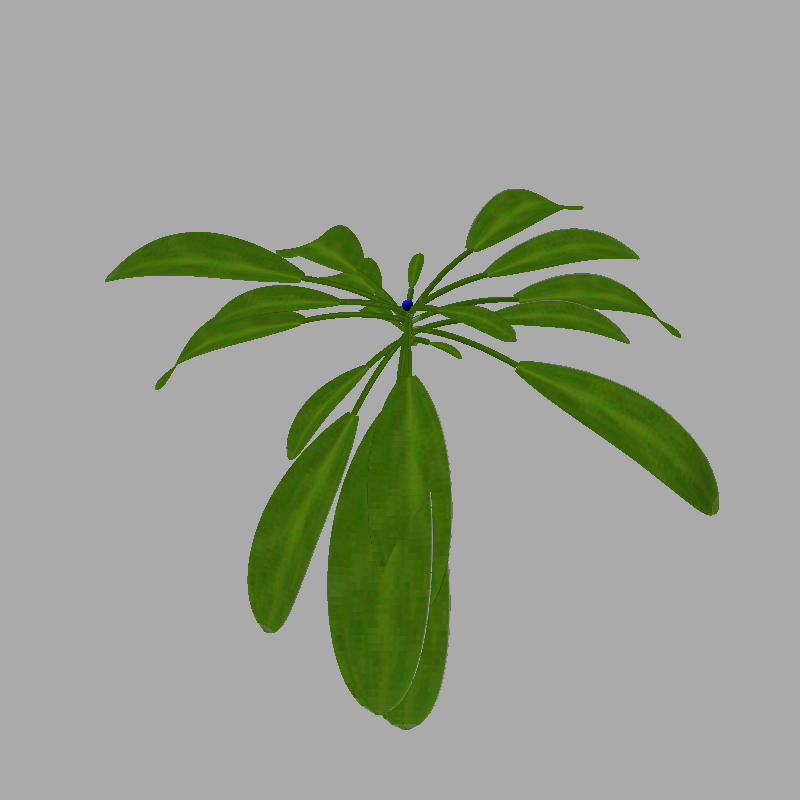
\includegraphics[width = 0.3\linewidth]{figures/10d.png}\hspace{1em}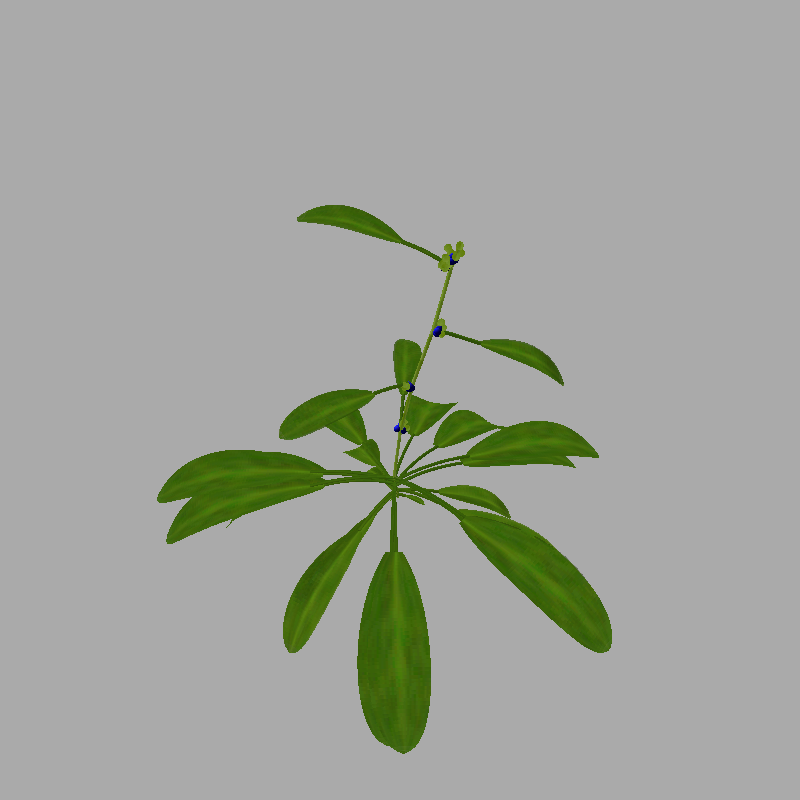
\includegraphics[width = 0.3\linewidth]{figures/20d.png}

    \vspace{0.9em}
    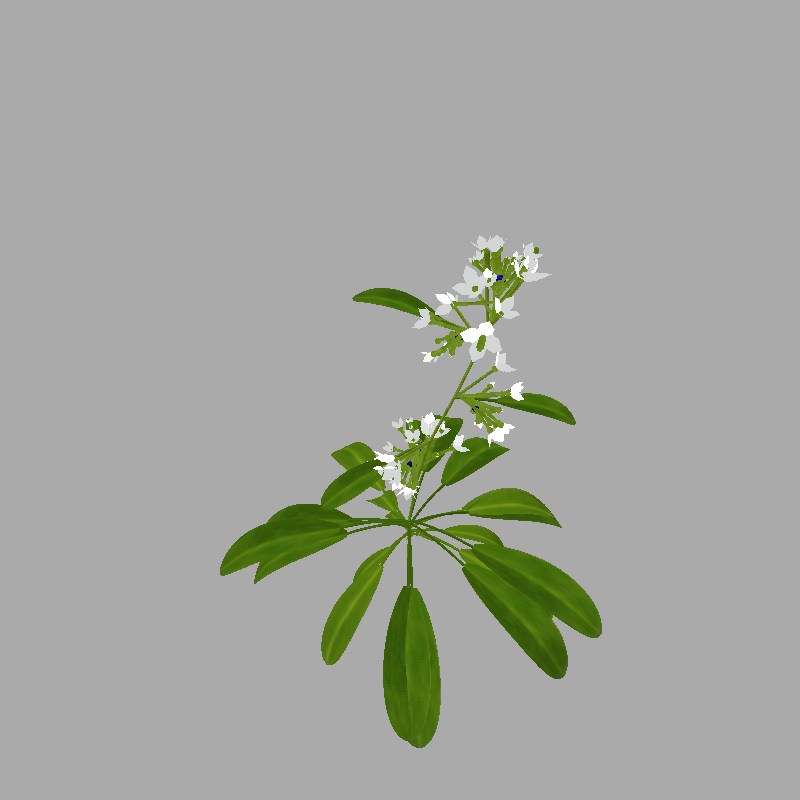
\includegraphics[width = 0.3\linewidth]{figures/30d.png}\hspace{1em}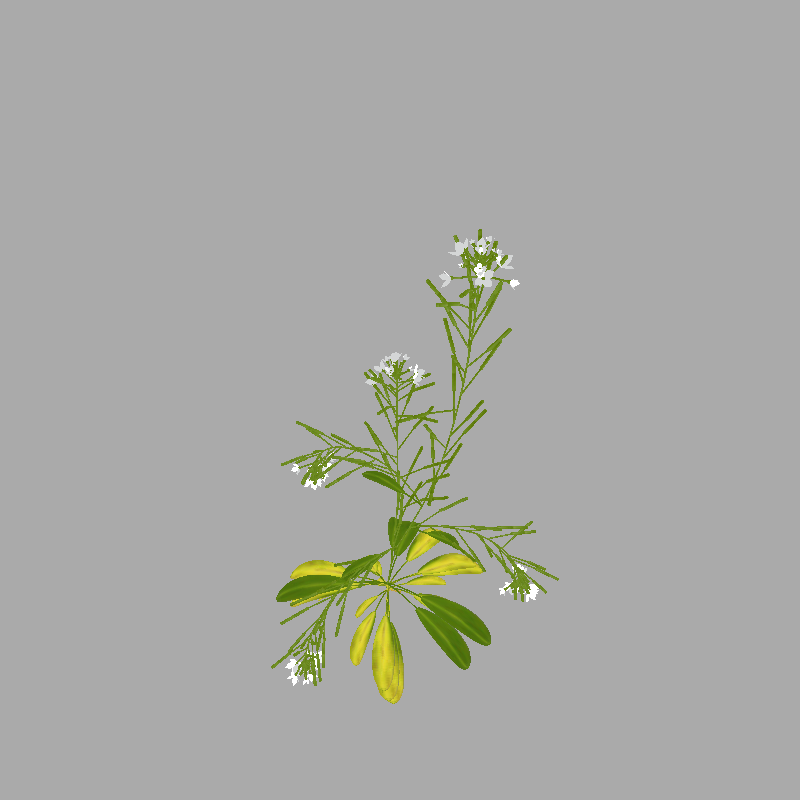
\includegraphics[width = 0.3\linewidth]{figures/40d.png}
    \caption{An example of simulated \emph{Arabidopsis thaliana} using L-py. The four figures are representation of the same
    simulation after 240 (top left), 480 (top right), 720 (bottom left) and 960 (bottom right) iterations of the
    L-system.} \label{fig:lpy}
\end{figure}


\tim{The generated plant models are exported as meshes using the
standard OBJ format.}{}

\paragraph{Virtual scanner.} \tim{The open source software
Blender~\cite{blender} was chosen for the rendering part. The blender
Eevee renderer allows for fast and realistic looking rendering of
scenes and the python bpy modules allows for easy scripting.}{}

\tim{The idea is to provide a simulated environment similar to
the real application described above.}{} \tim{A python script using bpy and
flask}{An API} was \tim{written}{implemented} to
generate and visualise the generated plant 3D models in Blender.
\tim{HTTP requests allow us to easily load different plant models and
backgrounds into the Blender scene, to move the loaded object,
as well as change the camera position, rotation and its intrinsic
parameters. The rendering of the scene into an image can also
be triggered by a simple request. This enables us to take pictures of the
model around the plant, as we would on the real world setup~(Figure
\ref{fig:plants}).}{The 3D models are loaded in a virtual environment
and virtual cameras are used to take pictures of the
model~(Figure \ref{fig:plants}).}

To further increase the diversity of the simulated dataset and prevent
overfitting on the chosen plant textures, random colors are taken
from a reference image and applied as the base color of the plant material.

\tim{The scene background }{The plant is placed in a virtual background. It} is a $360^{\circ}$
\tim{real world picture}{image} and rendering it in blender reproduces the
original scene lighting\tim{. In order to increase the complexity of the
images acquired with the virtual scanner, s}{S}everal sets of backgrounds were
used, without limitations on the lighting environement -- night, daylight,
sunset -- or the type of scene -- indoor or outdoor. A simulated flash light is
triggered with a random level of intensity to simulate different artifical lighting condition during the
acquisition of real life pictures.

\begin{figure}[h]
    \centering 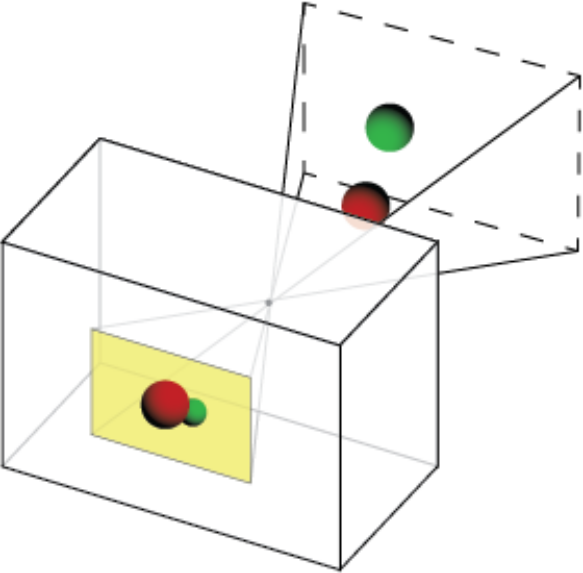
\includegraphics[width=0.3\linewidth]{figures/pinhole.png}
    \caption{Illustration of 2D overlapping due to perspective
    projection } \label{fig:pinhole}
\end{figure}

The \tim{ground truth plant part segmentation is}{virtual labels are} acquired by rendering the plant material by material, with one material per
\tim{plant part}{organ}~(Figure \ref{fig:plants}). The
\tim{plant parts}{organs} considered for \emph{A. Thaliana} are leaf, stem, flower,
fruit and peduncle. \tim{As we will see later for the 3D reconstruction, i}{I}n the pinhole model \cite{sturm_pinhole_2014} we use for 3D to 2D
projection, a whole line in 3D projects onto a single pixel (Figure
\ref{fig:pinhole}). As a consequence, a single pixel can belong to
several classes depending on the organs crossed by the line. The
labelling method takes this plurality into account by generating a
ground truth image for each class.

\begin{figure}[h]
    \centering 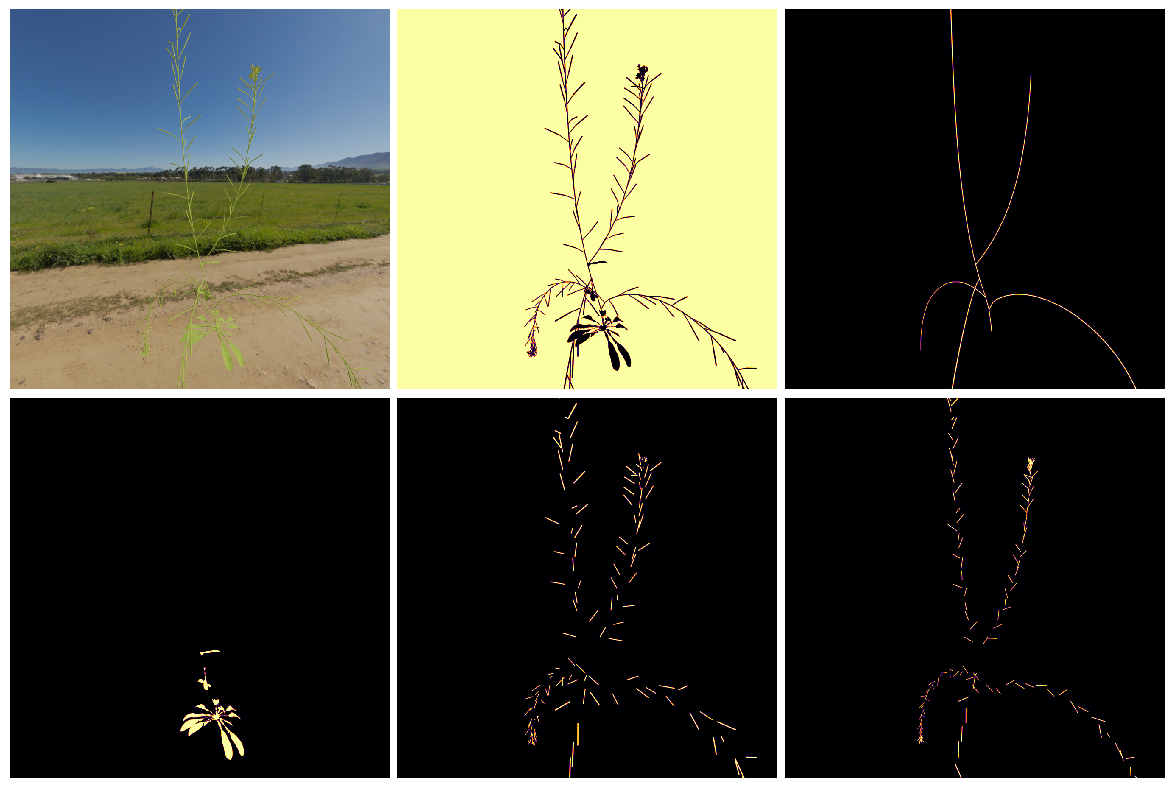
\includegraphics[width = 0.9\linewidth]{figures/Images_and_labels.png}
    \caption{Example of virtual training images and all labels}
    \label{fig:plants}
\end{figure}

\tim{The virtual scanner was used to generate a training dataset of plant
images with plant part segmentation 
for the training of neural networks.}{}


% \paragraph{3D ground truth.} The 3D virtual plants were
% used to train and evaluate the 3D reconstruction. The
% virtual mesh is regularly subsampled with CloudCompare
% \cite{girardeau-montaut_cloudcompare-open_2011} in order to get
% a density matching the voxel density in the volume to carve (see
% space carving section for explanations). Then this 3D point cloud is
% voxellized and each voxel of the volume to carve acquires an organ
% class, or class 0 (background) if it is not part of the plant. Then
% the vector is saved in a sparse representation to save memory. For the
% trainings, the data generator reads the sparse vector and encodes it
% in a dense representation to compare it to the predicted classes. It
% is needed to densify it because PyTorch can't backpropagate easily
% through a sparse representation.

%To train the classification on real plants, it was first considered
% to print a known plant model in 3D with Sculpteo, however the stem of
% the model wasn't thick enough and it buckled during the printing. We
% also considered to use an opensource dataset, however most segmented 3D
% dataset aimed for reconstruction are provided in Lidar or RGB-D data,
% and not from RGB to 3D. Therefore we decided to restrict ourselves to
% 3D virtual plants. We also used the 3D reconstructed models with the
% initial space-carving approach implemented previously in the pipeline
% \cite{wintz_automated_nodate} for comparison.


\paragraph{Image segmentation.} The objective of image \tim{semantic}{} segmentation is
to convert an input image in a stack of probability maps of the same
dimension as the image. \tim{If $C$ is the number of different classes,
semantic segmentation produces $C$ output images with values between $0$ and $1$,
giving for each pixel of the input image the probability of that pixel
belonging to the corresponding class.}{For C classes there will be C probability
maps, each corresponding to one class. The value of a pixel in the
probability map of class k is the probability that this pixel belongs
to the organ-type k in the original image.}


\tim{To produce such semantic probability maps, we used a segmentation
convolutional neural network~\cite{guo_review_2018}}{The image segmentation was performed using segmentation convolutional
neural network \cite{guo_review_2018}}. \tim{These}{Such} segmentation networks
are based on a contracting structure from an image to a low dimension\tim{al}{}
feature space, \tim{called the \emph{latent space}}{}, which encodes the content of the image. It is branched
to a symmetric expanding structure that translates the information from
the feature space to an image similar to the original one, but with
only the content of interest reconstructed. The contracting structure
is directly inspired from classification neural networks, and made
of convolution layers, non-linearities and down-pooling layers. The
convolution kernels allow to filter the information to emphasize
the content, and the down-pooling allows to reduce the dimension
of the information. The expanding structure reproduces the path in
the other direction, with up-pooling layers and convolutions. The
spatial information is re-injected to reconstruct the image properly,
by providing the down-pooling coordinates from the contracting phase.

\begin{figure}[h!]
    \centering 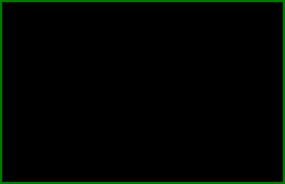
\includegraphics[scale = 0.25]{figures/blank.png}
    \caption{Example of segmentation network: the U-Net architecture
    \cite{ronneberger_u-net:_2015}} \label{fig:unet}
\end{figure}

\tim{We decided to use a neural network architecture inspired by}{The structure tested was inspired from}
U-Net~\cite{ronneberger_u-net:_2015}. However, \tim{to leverage the power of
already existing labeled datasets}{}, the contracting
structure, or encoder, was replaced by a classification network trained
on ImageNet, and with six classes to segment. \tim{Thanks to the great diversity
in the ImageNet dataset, t}{T}his classification
structure has already \tim{learned}{been trained} to encode the semantic
representation of an image in the latent space. \tim{The classification network that we used is}{We tested}
ResNet~\cite{he_deep_2015} which is a deep neural network where inputs
from previous layers are regularly reinjected into deeper layers
in order to maintain the geometry and avoid vanishing gradients
\cite{hochreiter_vanishing_1998}.

\paragraph{Training from simulated data.} The network was trained with
images from the virtual scanner. \alien{The training set consisted of 2520 images (896x896 pixels), 18 views of 140 different virtual models. The distance and position of the camera around the plant varied to offer more diversity.}{TODO(Describe the path, dimension of the images). The dataset comprised TODO(Number of images)} To make the network robust to images and lighting conditions that are not in the dataset, we artificially augment the dataset by adding \alien{gaussian noise ($\sigma$ = 0.01) and random rotations (Figure \ref{fig:trainset}). The images were normalized to correspond to the mean and variance of the training set of ImageNet, on which was initially trained the semantic structure (mean: $(0.485, 0.456, 0.406)$ standard-deviation: $(0.229, 0.224, 0.225)$)}{TODO(add gaussian noise, change contrast, rotation, déformation, more?).}. 
The dataset was split into 3 sets:

\begin{itemize}
    \item a training set to train the network (70\% of the dataset)
    \item a validation set on which the network is not trained and
    is used to evaluate and compare the different networks (7\%
    of the dataset) \item a test set used at the very end on the
    selected architecture (23\% of the dataset)
\end{itemize}

\begin{figure}[h!]
	\centering 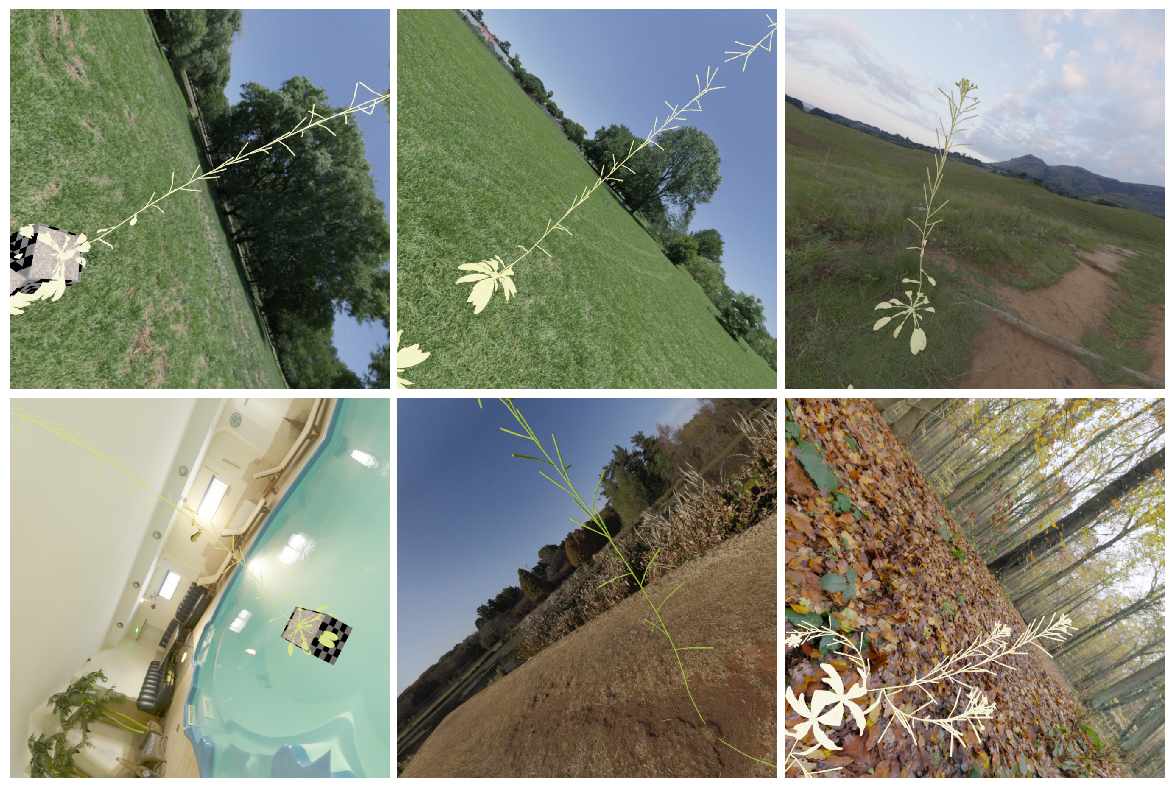
\includegraphics[width = 0.9\linewidth]{figures/vscan_sample.png}
	\caption{Sample of the training set (before normalization)} \label{fig:trainset}
\end{figure}


To evaluate the segmentation of the images, a combination of
metrics were used. As it is a multiclass problem, a sigmoid is
applied to each output in order to contain the numerical range of
the predictions. First crossentropy was used, it is a per-pixel
metric. It represents the uncertainty of the prediction compared to
the ground-truth. If the class of a pixel has a very low predicted
probability, it will highly penalise the loss. If the probability
is close to one, the contribution to the loss is close to zero. The
notion of entropy represents this discrepancy between the ground truth
distribution and the predicted distribution. It is naturally translated
at the mathematical level with the negative of the logarithm.

\begin{equation}
    L =-\sum_i^n\sum_k^C{y^k_{i, gt}\ln(y_{\textrm{i},
    \textrm{pred}}^k)}
\end{equation}

Where n is the number of pixels in the image, C the number of possible
classes, $y_{gt}^k = 1$ if pixel i is in class k, 0 otherwise, and
$y_ {\textrm{i}, \textrm{pred}}^k = p(\textrm{label}(y_{\textrm{i},
\textrm{gt}}) = k)$.

The second loss we used was the Dice coefficient, which theoretically
writes as:

\begin{equation}
    s = 1 - \frac{1}{n}\sum_{i=1}^n\sum_{k=0}^{C}y_{\textrm{i},
    \textrm{gt}} y_{\textrm{i}, \textrm{pred}}^k
\end{equation}


This coefficient compares the number of right predictions to the
number of samples, for each class. In practice, the product of the
ground truth by the predictions is summed, so that only the prediction
of the right class contributes to the sum. For example for point n,
the class is k, and the prediction for class k is $p_k$, the loss
for point n will be $1 - \frac{2p_k}{2} = 1 - p_k$. The total loss
is computed vector-wise, and lies between 0 and 1.


We used the mean of these two losses for the training, as the
crossentropy has more stable gradients, but the Dice loss is what we
want to minimise, and is less sensitive to class imbalance.


\paragraph{Fine-tuning.} Our network was trained on virtual \emph{A.
Thaliana} model but aims at reconstructing real plants. \alien{Although the training performs well for real \emph{A. Thaliana}, it transfers poorly to other species with large anatomical differences. }{Therefore when
the virtual plants fail at reproducing the complexity of real plants,
the network can perform poorly. The network also fails when confronted
to other plant species with very different traits.} Therefore we
conceived a simple interface that allows the user to manually label a
few images of interest (two or three images is enough), then run the training
of the network on this small dataset. This way, the network will be
able to segment similar images with correct classes.
\alien{The interface uses LabelMe \cite{russell_labelme:_2008} for manual annotations, and runs the training on these images for 20 epochs. This generates a segmentation network specialized for the new species, starting from the network trained on the virtual plant models of \emph{A. Thaliana}.}{}

\paragraph{Structure from motion.} To map points in space to their location in each
individual pictures, one has to know the precise intrinsic camera models as well
as the exact position of cameras in space. In a simulation environment,
these can be computed and stored as picture metadata, but it is rather
challenging to perfectly calibrate a camera arm in real world scenarios. Thus,
we propose to obtain camera poses using a structure from motion algorithm -- in
this work, we used the open source software Colmap~\cite{schoenberger2016mvs,
schoenberger2016sfm}. Structure from motion is a well known algorithm which
allows us to automatically obtain camera poses from a set of rgb pictures, up to
a scaling of the world. The scaling coefficient is then obtained either
approximately using the translation parameter of the camera arm, or more
precisely using a custom calibration procedure. (TODO: see annex? uwritten article?)

If $N$ is the number of views taken of a given scene,
we thus have projection models -- including both intrinsic camera parameters
and camera pose estimation -- $\pi_i : \mathbb{R}^3 \rightarrow \mathbb{R}^2,i \in \{1,\cdots, N\}$,
such that for any world coordinates $x \in \mathbb{R}^3$, $\pi_i ({x})$ is the
pixel coordinate of point ${x}$ in view $i$.

\paragraph{Space Carving.} We combine the background class and the space carving
approach to obtain the geometry of points in space. Space carving~\cite{kutulakos_theory_1999}
is a photogrammetric approach which uses
pictures of an object from different point of views to reconstruct
an object in 3D as a binary function of space. Space is divided into a regular voxel grid with a voxel size chosen
such that the size of the projection of each voxel is of the same order of magnitude of a pixel in each
if the pictures. Algorithm~\ref{algorithm:sc} details the space carving method.

The resulting set of voxels whose value is \emph{seen} correspond to the
\emph{visual hull} of the object under the given views, and is an approximation
of the true volume occupied by the object in space. To compute a point cloud
from this volume, a level set method is used, as described in
algorithm~\ref{algorithm:pcdn}. The signed distance function needed for this algorithm is computed using a
fast marching algorithm in scipy~\ref{scipy}. This yields a set of point located on the  
surface of the interface between the inside and the outside of the visual hull.

\begin{algorithm}
    \caption{Space carving algorithm}
    \label{algorithm:sc}
    \begin{algorithmic}[1]
        \Function{SpaceCarving}{$V, \Omega, B_1, \pi_1, B_2, \pi_2, \dots, B_N, \pi_N$}

        \Comment{$V$ is a set of voxels, each having a value and a center.}
        \Comment{$B_i$ is a mask indicating background $B_i(x) == 1$ iff pixel
$x$ is classified as background.}
        \Comment{$\pi_i$ is the projection from world coordinates to pixel
coordinates.}
        \Comment{$\Omega = [0,w] \times [0,h]$ is the image domain.}

        \For{$v \in V$}
            $v.\textrm{value} \gets \textrm{unseen}$
        \EndFor{}
        \For{$i \in 1, \cdots, N$}
            \For{$v \in V$}
                \If{$\pi_i(v) \in \Omega$}
                    \If{$B_1[\pi_i(v)] == 1$}
                        $v.\textrm{value} \gets \textrm{background}.$
                    \ElsIf{$v.\textrm{value} == \textrm{unseen}$}
                        $v.\textrm{value} \gets \textrm{seen}.$
                    \EndIf{}
                \EndIf{}
            \EndFor{}
        \EndFor{}
        \EndFunction
    \end{algorithmic}
\end{algorithm}

\begin{algorithm}
    \caption{From voxel grid to point cloud}
    \label{algorithm:pcdn}
    \begin{algorithmic}[1]
        \Function{PointCloud}{V}
        \State $D \gets \Call{SignedDistance}{V == 1}$
        \State $\nabla D \gets \Call{Gradient}{D}$
        \State $points \gets []$
        \State $normals \gets []$
        \For{$v \in V : |D[v]| < \sqrt{2} / 2$ }

        \Comment{Loop on all boundary points.}
            \State $n \gets \nabla D [v] / \Vert \nabla D [v] \Vert$
            \State $v_1 \gets v + D[v] * n$
            \State $\Call{Append}{points, v_1}$
            \State $\Call{Append}{normals, n}$
        \EndFor{}
        \State \textbf{return} $points, normals$
        \EndFunction
    \end{algorithmic}
\end{algorithm}

\paragraph{Backprojection. }

The following task is to attribute a label to each point in the point cloud
computed with the previous step. To do so, similarly to the space carving
method, each point is projected onto segmented images.

Let $M_{i,k}$ denote the output of the segmentation algorithm for view $i$ and
class $k$. In the following, classes include all non-background organ classes.
A threshold is applied to the probability scores, so that $M_{i,k} (x) \in \{0,
1\}$ for all $x$ in $\Omega$. Then, for each point, each class gets a vote from each of its
projection in the masks $M_{i,k}$:

$$
M_k(x) = \sum_{i\in I(x)} M_{i,k} (\pi_i(x) ).
$$

Then the class with the maximal number of votes is attributed to the point:

$$
\textrm{class}(x) = \textrm{argmax}_k ( M_k(x) ).
$$

If a point gets no vote from any of its projection, then it is discarded as a
background point.  This yields a labeled point cloud, such that every point in
it is attributed a non-background class.
